\documentclass[]{ximera}
%handout:  for handout version with no solutions or instructor notes
%handout,instructornotes:  for instructor version with just problems and notes, no solutions
%noinstructornotes:  shows only problem and solutions

%% handout
%% space
%% newpage
%% numbers
%% nooutcomes

%I added the commands here so that I would't have to keep looking them up
%\newcommand{\RR}{\mathbb R}
%\renewcommand{\d}{\,d}
%\newcommand{\dd}[2][]{\frac{d #1}{d #2}}
%\renewcommand{\l}{\ell}
%\newcommand{\ddx}{\frac{d}{dx}}
%\everymath{\displaystyle}
%\newcommand{\dfn}{\textbf}
%\newcommand{\eval}[1]{\bigg[ #1 \bigg]}

%\begin{image}
%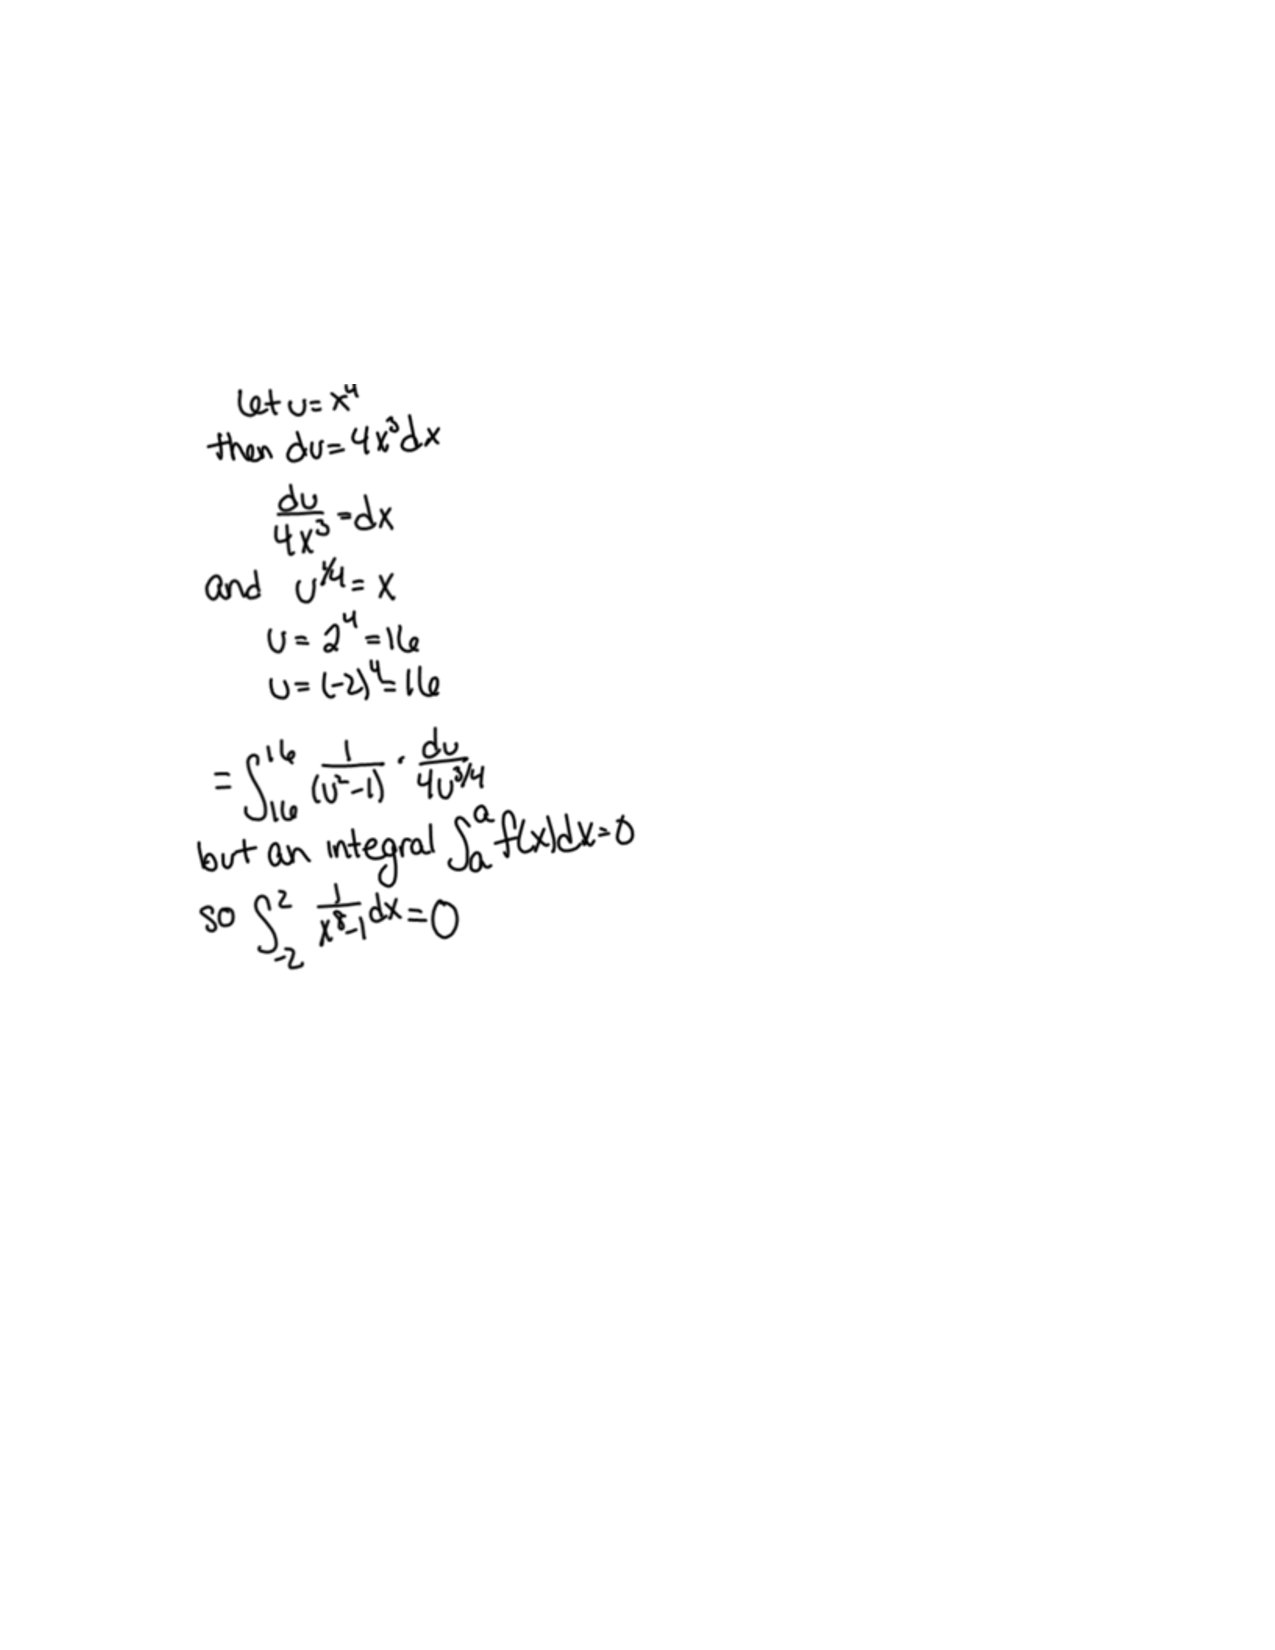
\includegraphics[trim= 170 420 250 180]{Figure1.pdf}
%\end{image}

%add a ``.'' below when used in a specific directory.
\newcommand{\RR}{\mathbb R}
\renewcommand{\d}{\,d}
\newcommand{\dd}[2][]{\frac{d #1}{d #2}}
\renewcommand{\l}{\ell}
\newcommand{\ddx}{\frac{d}{dx}}
\newcommand{\dfn}{\textbf}
\newcommand{\eval}[1]{\bigg[ #1 \bigg]}

\usepackage{multicol}

\renewenvironment{freeResponse}{
\ifhandout\setbox0\vbox\bgroup\else
\begin{trivlist}\item[\hskip \labelsep\bfseries Solution:\hspace{2ex}]
\fi}
{\ifhandout\egroup\else
\end{trivlist}
\fi} %% we can turn off input when making a master document

\title{Physical applications}  

\begin{document}
\begin{abstract}		\end{abstract}
\maketitle



\begin{comment}
\section{Warm up:}

	\begin{freeResponse}
	
	\end{freeResponse}
	
\begin{instructorNotes}

\end{instructorNotes}
\end{comment}







\section{Group work:}



%problem 1
\begin{problem}
A metal bar $8$ meters long has density (in kg/m) $x$ meters from the left end of the bar given by
	\begin{equation*}
	\rho(x) = \left\{ \begin{array}{rl} x^2 & \quad \text{if } 0 \leq x \leq 3 \\ \frac{4}{x} & \quad \text{if } 3 < x \leq 8. \end{array} \right.  
	\end{equation*}
Find the mass of the portion of the bar from $2$ meters to $5$ meters from its left end.
	
	\begin{freeResponse}
		\begin{align*}
		\text{{\color{red} mass}} &= \int_a^b \rho(x) \d x  \\
		&= \int_2^3 \rho(x) \d x + \int_3^5 \rho(x) \d x  \\
		&= \int_2^3 x^2 \d x + \int_3^5 \frac{4}{x} \d x  \\
		&= \eval{\frac{1}{3} x^3}_2^3 + \eval{4 \ln|x|}_3^5  \\
		&= \left( 9 - \frac{8}{3} \right) + \left(4 \ln (5) - 4 \ln (3) \right)  \\
		&= \left( \frac{19}{3} + 4 \ln \left( \frac{5}{3} \right) \right) \, kg.
		\end{align*}
	\end{freeResponse}
	
\end{problem}

\begin{instructorNotes}
There are currently no instructor notes for any of the problems in this section (there was no teaching guide posted).
\end{instructorNotes}







%problem 2
\begin{problem}
Assume that a spring, whose equilibrium length is $1$ meter, obeys Hooke's law.
It requires $25J$ of work to compress this spring to $0.7m$ in length.  
	\begin{enumerate}
		\item  Find the work required to compress the spring to $0.6m$ in length.  
		\begin{freeResponse}
		Let $W$ denote the amount of work done.  
		Recall that
			\[
			W = \int_a^b F(x) \d x
			\]
		where $F$ denotes the variable force applied to move the object (in a straight line) from $x=a$ to $x=b$ in the direction of the force.  
		Recall that Hooke's law says that
			\[
			F(x) = k x
			\]
		where $k$ is a constant that depends only on the spring.  
		
		To solve this problem, we first need to solve for $k$.  
		Using the given information, we have that
			\begin{align*}
			25 \, J &= \int_0^{-0.3} kx \d x  \\
			&= \eval{\frac{k}{2} x^2}_0^{-0.3}  \\
			&= \frac{k}{2} (0.09 - 0) = \frac{9k}{200}
			\end{align*}
		and so
			\[
			k = \frac{200}{9} \cdot 25 = \frac{5000}{9} \, \frac{N}{m}.
			\]
			
		Now, to answer part (a), we evaluate the integral
			\begin{align*}
			W &= \int_0^{-0.4} \frac{5000}{9} x \d x  \\
			&= \eval{\frac{2500}{9} x^2}_0^{-0.4}  \\
			&= \frac{2500}{9} \cdot \left( \frac{2}{5} \right)^2   \\
			&= \left( \frac{2500}{9} \right) \left( \frac{4}{25} \right) = \frac{400}{9} \, J
			\end{align*}
		\end{freeResponse}
		
		
		
		\item  Find the work required to stretch the spring from $1.4m$ to $1.8m$.
		\begin{freeResponse}
			\begin{align*}
			W &= \int_{0.4}^{0.8} k x \d x  \\
			&= \frac{5000}{9} \int_{0.4}^{0.8} x \d x \qquad \text{{\color{red} we know k from part (a) }}\\
			&= \eval{\frac{2500}{9} x^2}_{0.4}^{0.8}  \\
			&= \frac{2500}{9} \left( \frac{16}{25} - \frac{4}{25} \right)  \\
			&= \frac{400}{3} \, J.
			\end{align*}
		\end{freeResponse}
		
	\end{enumerate}
		
\end{problem}

\begin{instructorNotes}

\end{instructorNotes}







%problem 3
\begin{problem}
A bucket with mass $100kg$ when filled with oil is lifted at a constant rate by a pulley from the bottom to the top of a $60$-meter hole.
	\begin{enumerate}
		\item  Assuming the chain used to lift the bucket has negligible mass, compute the work needed to lift the bucket from the bottom of the hole to the top.  
		\begin{freeResponse}
		Let
			\begin{align*}
			m &= \text{ mass } = 100 \, kg  \\
			g &= \text{ gravitational constant }  \\
			y &= \text{ height } = 60 \, m  \\
			W &= \text{ work}.
			\end{align*}
		Then
			\[
			W = m \cdot g \cdot y = 6000 g
			\]
		\end{freeResponse}
		
		
		
		\item  Assuming the chain used to lift the bucket has an evenly-distributed mass of $12kg$, set up an integral that will compute the amount of work needed to lift the bucket from the bottom to the top of the hole.  
		\begin{freeResponse}
		First notice that
			\begin{align*}
			\text{{\color{red}Total Work} } &= \text{ work to lift the bucket } + \text{ work to lift the chain}  \\
			&= 6000 g + \text{ work to lift the chain}.
			\end{align*}
		
		Next, the weight of the chain has an even distribution of $\rho = \frac{12}{60} = \frac{1}{5} \cdot \frac{kg}{m}$.  
		Also, at any generic height $y$, the remaining distance that this link in the chain needs to be raised is $(60-y)$.  
		Thus, we have
			\begin{align*}
			\text{work to lift the chain } &= \int_0^{60} \frac{1}{5} (60-y) g \d y  \\
			&= \frac{g}{5} \int_0^{60} (60-y) \d y  \\
			&= \frac{g}{5} \eval{60y - \frac{1}{2} y^2}_0^{60}  \\
			&= \frac{g}{5} \left( 3600 - 1800 \right) = 360g.
			\end{align*}
		Therefore
			\[
			W = 6000g + 360g = 6360g.
			\]
		\end{freeResponse}
		
		
		
		\item  Assuming the chain used to lift the bucket has an evenly-distributed mass of $12kg$ {\it and} that oil is leaking out of a hole in the bucket at a constant rate such that the bucket and the remaining oil has a mass of $27kg$ when it reaches the top, set up an integral that will compute the amount of work to lift the bucket from the bottom of the hole to the top (assuming that the bucket is lifted at a constant rate).
		\begin{freeResponse}
		Similar to part (b), we have that
			\begin{align*}
			\text{{\color{red}Total Work} } &= \text{ work to lift the bucket } + \text{ work to lift the chain}  \\
			&= \text{ work to lift the bucket } + 360g.
			\end{align*}
		Now, when $y=0$ the mass of the bucket is $100 kg$.  
		When $y=60$ the mass of the bucket is $27kg$.  
		So the bucket loses $\frac{73}{60} kg$ of mass per meter.  
		Thus, the mass of the bucket at height $y$ is $100 - \frac{73}{60} y$.  
		
		Then
			\begin{align*}
			\text{work to lift the bucket } &= \int_0^{60} \left(100 - \frac{73}{60} y \right) g \d y  \\
			&= g \eval{100y - \frac{73}{120} y^2 }_0^{60}  \\
			&= g (6000 - 2190) = 3810 g.
			\end{align*}
		Therefore
			\[
			W = 3810g + 360g = 4170g.
			\]
		\end{freeResponse}
		
	\end{enumerate}

\end{problem}

\begin{instructorNotes}

\end{instructorNotes}







%problem 4
\begin{problem}
A truncated conical tank that is $8$ feet tall, $5$ feet across the top, and $3$ feet across the bottom is filled with water (water weighs $62.5$ pounds per cubic foot).  
\begin{enumerate}
		\item  Set up an integral that will compute the work needed to pump the water out of the top of the tank.  
		\begin{freeResponse}
			\begin{image}
			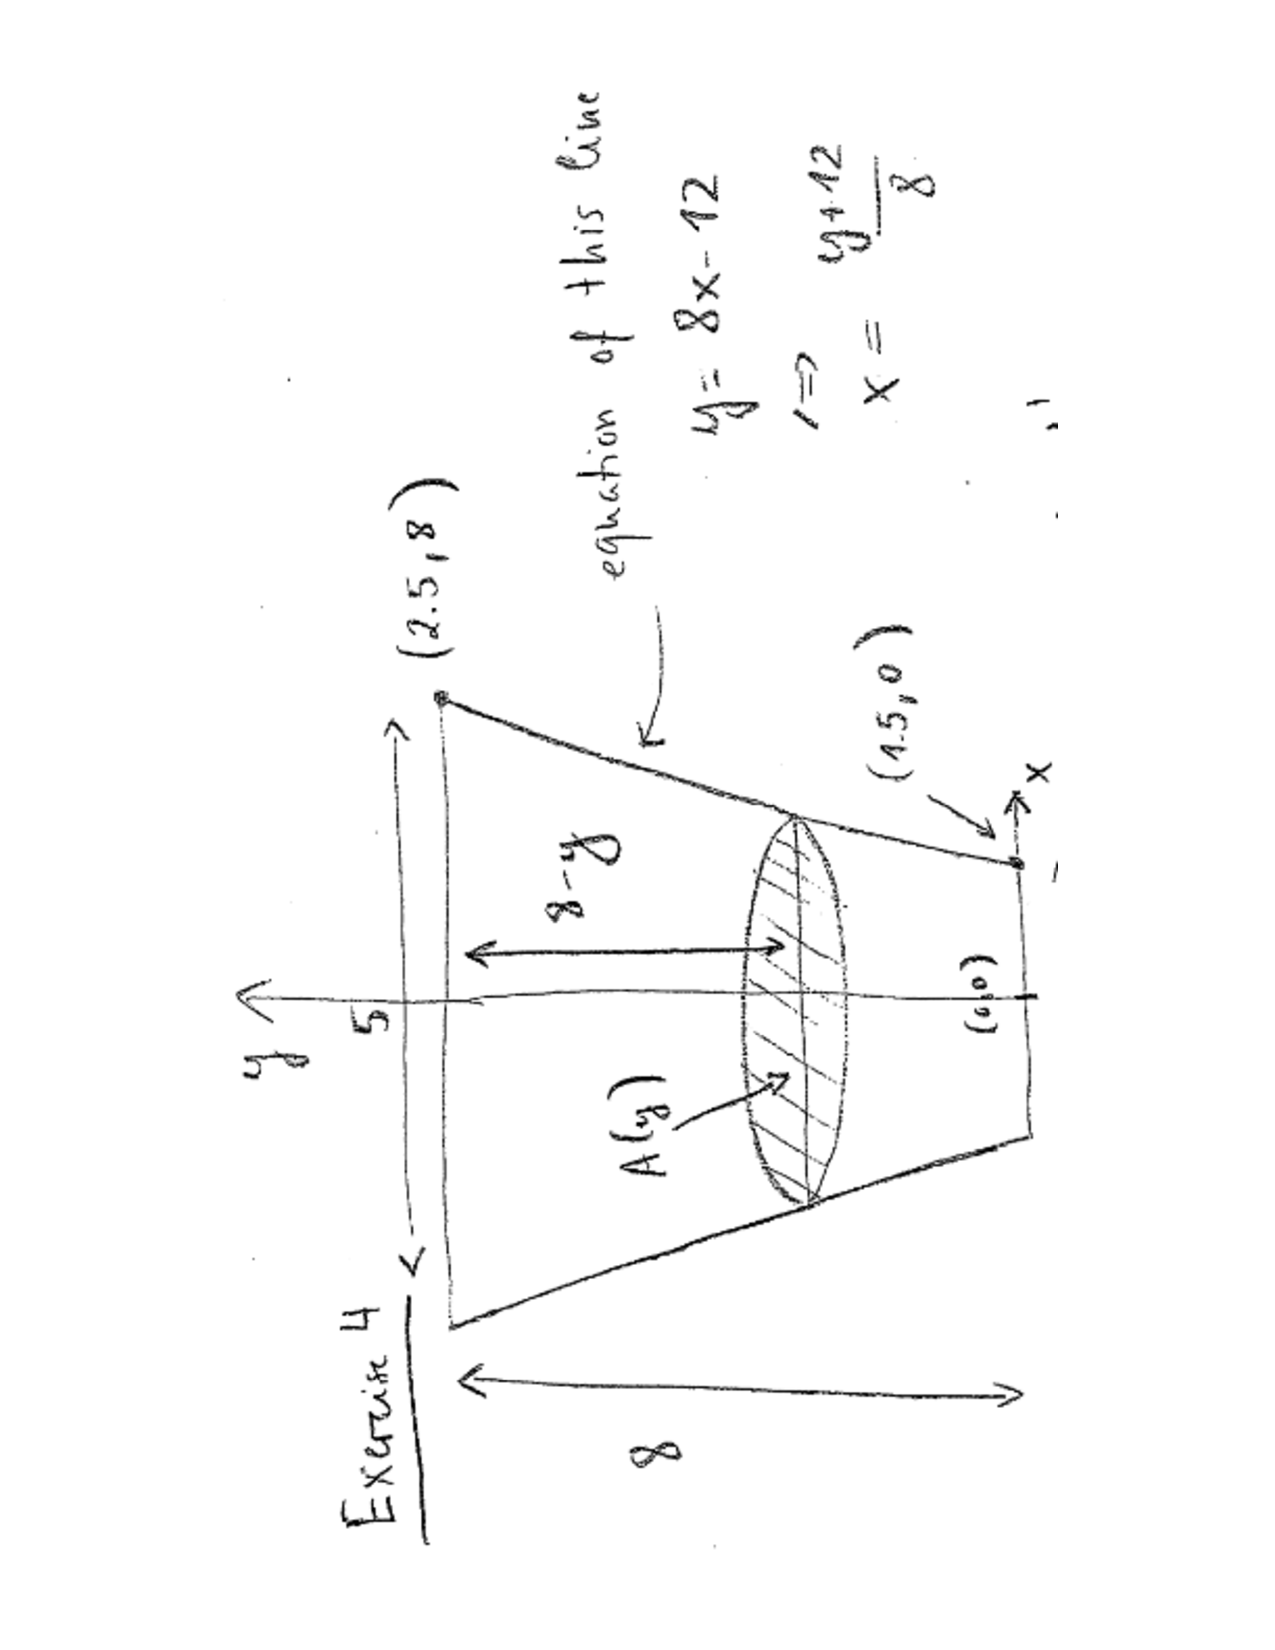
\includegraphics[trim= 120 320 100 180, angle=-89.99, scale=0.6]{Figure6-7-1.pdf}
			\end{image}
		
		Note that
			\begin{align*}
			\rho \times g&= 62.5,  \\
			\text{where} \rho &= \text{density}, \\
			g &= \text{ gravitational constant}  \\
			D(y) &= 8-y  \\
			A(y) &= \pi r^2 = \pi x^2 = \pi \left( \frac{y+12}{8} \right)^2.
			\end{align*}
		
		So
			\begin{align*}
			W &= \int_a^b \rho g A(y) D(y) \d y  \\
			&= 62.5 \pi \int_0^8 \left( \frac{y+12}{8} \right)^2 (8-y) \d y.
			\end{align*}
		\end{freeResponse}
		
		
		
		\item  Set up an integral that will compute the work needed to pump the water out of a pipe that sticks $2$ feet above the top of the tank.
		\begin{freeResponse}
		Since the pump is now $10 ft$ away from the point $(0,0)$ instead of $8 ft$, we just replace $D(y) = 8-y$ by $D(y) = 10-y$.  
		So
			\begin{align*}
			W &= \int_a^b \rho g A(y) D(y) \d y  \\
			&= 62.5 \pi \int_0^8 \left( \frac{y+12}{8} \right)^2 (10-y) \d y.
			\end{align*}
		\end{freeResponse}
		
	\end{enumerate}

\end{problem}

\begin{instructorNotes}

\end{instructorNotes}
















	
	
	
	
	
	
	
	
	

	










								
				
				
	














\end{document} 


















